\documentclass[12pt,twoside]{article}
\usepackage[dvipsnames]{xcolor}
\usepackage{tikz,graphicx,amsmath,amsfonts,amscd,amssymb,mathrsfs, bm,cite,epsfig,epsf,url}
\usepackage[hang,flushmargin]{footmisc}
\usepackage[colorlinks=true,urlcolor=blue,citecolor=blue]{hyperref}
\usepackage{amsthm,multirow,wasysym,appendix}
\usepackage{array,subcaption} 
% \usepackage[small,bf]{caption}
\usepackage{bbm}
\usepackage{pgfplots}
\usetikzlibrary{spy}
\usepgfplotslibrary{external}
\usepgfplotslibrary{fillbetween}
\usetikzlibrary{arrows,automata}
\usepackage{thmtools}
\usepackage{blkarray} 
\usepackage{textcomp}
\usepackage{float}
%\usepackage[left=0.8in,right=1.0in,top=1.0in,bottom=1.0in]{geometry}


\usepackage{times}
\usepackage{amsfonts}
\usepackage{amsmath}
\usepackage{latexsym}
\usepackage{color}
\usepackage{graphics}
\usepackage{enumerate}
\usepackage{amstext}
\usepackage{blkarray}
\usepackage{url}
\usepackage{epsfig}
\usepackage{bm}
\usepackage{hyperref}
\hypersetup{
    colorlinks=true,
    linkcolor=blue,
    filecolor=magenta,      
    urlcolor=blue,
}
\usepackage{textcomp}
%\usepackage[left=0.8in,right=1.0in,top=1.0in,bottom=1.0in]{geometry}
\usepackage{mathtools}
%\usepackage{minted}
\usepackage{gensymb}

%% Probability operators and functions
%
% \def \P{\mathrm{P}}
\def \P{\mathrm{P}}
\def \E{\mathrm{E}}
\def \Var{\mathrm{Var}}
\let\var\Var
\def \Cov {\mathrm{Cov}} \let\cov\Cov
\def \MSE {\mathrm{MSE}} \let\mse\MSE
\def \sgn {\mathrm{sgn}}
\def \R {\mathbb{R}}
\def \C {\mathbb{C}}
\def \N {\mathbb{N}}
\def \Z {\mathbb{Z}}
\def \cV {\mathcal{V}}
\def \cS {\mathcal{S}}

\newcommand{\RR}{\ensuremath{\mathbb{R}}}

\DeclareMathOperator*{\argmin}{arg\,min}
\DeclareMathOperator*{\argmax}{arg\,max}
\newcommand{\red}[1]{\textcolor{red}{#1}}
\newcommand{\blue}[1]{\textcolor{blue}{#1}}
\newcommand{\green}[1]{\textcolor{ForestGreen}{ #1}}
\newcommand{\fuchsia}[1]{\textcolor{RoyalPurple}{ #1}}



%
%% Probability distributions
%
%\def \Bern    {\mathrm{Bern}}
%\def \Binom   {\mathrm{Binom}}
%\def \Exp     {\mathrm{Exp}}
%\def \Geom    {\mathrm{Geom}}
% \def \Norm    {\mathcal{N}}
%\def \Poisson {\mathrm{Poisson}}
%\def \Unif    {\mathrm {U}}
%
\DeclareMathOperator{\Norm}{\mathcal{N}}

\newcommand{\bdb}[1]{\textcolor{red}{#1}}

\newcommand{\ml}[1]{\mathcal{ #1 } }
\newcommand{\wh}[1]{\widehat{ #1 } }
\newcommand{\wt}[1]{\widetilde{ #1 } }
\newcommand{\conj}[1]{\overline{ #1 } }
\newcommand{\rnd}[1]{\tilde{ #1 } }
\newcommand{\rv}[1]{ \rnd{ #1}  }
\newcommand{\rx}{\rnd{ x}  }
\newcommand{\ry}{\rnd{ y}  }
\newcommand{\rz}{\rnd{ z}  }
\newcommand{\ra}{\rnd{ a}  }
\newcommand{\rb}{\rnd{ b}  }
\newcommand{\rpc}{\widetilde{ pc}  }
\newcommand{\rndvec}[1]{\vec{\rnd{#1}}}

\def \cnd {\, | \,}
\def \Id { I }
\def \J {\mathbf{1}\mathbf{1}^T}

\newcommand{\op}[1]{\operatorname{#1}}
\newcommand{\setdef}[2]{ := \keys{ #1 \; | \; #2 } }
%\newcommand{\set}[2]{ \keys{ #1 \; | \; #2 } }
\newcommand{\sign}[1]{\op{sign}\left( #1 \right) }
\newcommand{\trace}[1]{\op{tr}\left( #1 \right) }
\newcommand{\tr}[1]{\op{tr}\left( #1 \right) }
\newcommand{\inv}[1]{\left( #1 \right)^{-1} }
%\newcommand{\abs}[1]{\left| #1 \right|}
\newcommand{\sabs}[1]{| #1 |}
\newcommand{\keys}[1]{\left\{ #1 \right\}}
\newcommand{\sqbr}[1]{\left[ #1 \right]}
\newcommand{\sbrac}[1]{ ( #1 ) }
\newcommand{\brac}[1]{\left( #1 \right) }
\newcommand{\bbrac}[1]{\big( #1 \big) }
\newcommand{\Bbrac}[1]{\Big( #1 \Big)}
\newcommand{\BBbrac}[1]{\BIG( #1 \Big)}
\newcommand{\MAT}[1]{\begin{bmatrix} #1 \end{bmatrix}}
\newcommand{\sMAT}[1]{\left(\begin{smallmatrix} #1 \end{smallmatrix}\right)}
\newcommand{\sMATn}[1]{\begin{smallmatrix} #1 \end{smallmatrix}}
\newcommand{\PROD}[2]{\left \langle #1, #2\right \rangle}
\newcommand{\PRODs}[2]{\langle #1, #2 \rangle}
\newcommand{\der}[2]{\frac{\text{d}#2}{\text{d}#1}}
\newcommand{\pder}[2]{\frac{\partial#2}{\partial#1}}
\newcommand{\derTwo}[2]{\frac{\text{d}^2#2}{\text{d}#1^2}}
\newcommand{\ceil}[1]{\lceil #1 \rceil}
\newcommand{\Imag}[1]{\op{Im}\brac{ #1 }}
\newcommand{\Real}[1]{\op{Re}\brac{ #1 }}
%\newcommand{\norm}[1]{\left|\left| #1 \right|\right| }
\newcommand{\norms}[1]{ \| #1 \|  }
\newcommand{\normProd}[1]{\left|\left| #1 \right|\right| _{\PROD{\cdot}{\cdot}} }
\newcommand{\normTwo}[1]{\left|\left| #1 \right|\right| _{2} }
\newcommand{\normTwos}[1]{ \| #1  \| _{2} }
\newcommand{\normZero}[1]{\left|\left| #1 \right|\right| _{0} }
\newcommand{\normTV}[1]{\left|\left| #1 \right|\right|  _{ \op{TV}  } }% _{\op{c} \ell_1} }
\newcommand{\normOne}[1]{\left|\left| #1 \right|\right| _{1} }
\newcommand{\normOnes}[1]{\| #1 \| _{1} }
\newcommand{\normOneTwo}[1]{\left|\left| #1 \right|\right| _{1,2} }
\newcommand{\normF}[1]{\left|\left| #1 \right|\right| _{\op{F}} }
\newcommand{\normLTwo}[1]{\left|\left| #1 \right|\right| _{\ml{L}_2} }
\newcommand{\normNuc}[1]{\left|\left| #1 \right|\right| _{\ast} }
\newcommand{\normOp}[1]{\left|\left| #1 \right|\right|  }
\newcommand{\normInf}[1]{\left|\left| #1 \right|\right| _{\infty}  }
\newcommand{\proj}[1]{\mathcal{P}_{#1} \, }
\newcommand{\diff}[1]{ \, \text{d}#1 }
\newcommand*\Diff[1]{\mathop{}\!\mathrm{d^#1}}
\newcommand{\vc}[1]{\boldsymbol{\vec{#1}}}
\newcommand{\rc}[1]{\boldsymbol{#1}}
\newcommand{\vx}{\vec{x}}
\newcommand{\vy}{\vec{y}}
\newcommand{\vz}{\vec{z}}
\newcommand{\vu}{\vec{u}}
\newcommand{\vv}{\vec{v}}
\newcommand{\vb}{\vec{\beta}}
\newcommand{\va}{\vec{\alpha}}
\newcommand{\vaa}{\vec{a}}
\newcommand{\vbb}{\vec{b}}
\newcommand{\vg}{\vec{g}}
\newcommand{\vw}{\vec{w}}
\newcommand{\vh}{\vec{h}}
\newcommand{\vbeta}{\vec{\beta}}
\newcommand{\valpha}{\vec{\alpha}}
\newcommand{\vgamma}{\vec{\gamma}}
\newcommand{\veta}{\vec{\eta}}
\newcommand{\vnu}{\vec{\nu}}
\newcommand{\rw}{\rnd{w}}
\newcommand{\rvnu}{\vc{\nu}}
\newcommand{\rvv}{\rndvec{v}}
\newcommand{\rvw}{\rndvec{w}}
\newcommand{\rvx}{\rndvec{x}}
\newcommand{\rvy}{\rndvec{y}}
\newcommand{\rvz}{\rndvec{z}}
\newcommand{\rvX}{\rndvec{X}}


\newtheorem{theorem}{Theorem}[section]
% \declaretheorem[style=plain,qed=$\square$]{theorem}
\newtheorem{corollary}[theorem]{Corollary}
\newtheorem{definition}[theorem]{Definition}
\newtheorem{lemma}[theorem]{Lemma}
\newtheorem{remark}[theorem]{Remark}
\newtheorem{algorithm}[theorem]{Algorithm}

% \theoremstyle{definition}
%\newtheorem{example}[proof]{Example}
\declaretheorem[style=definition,qed=$\triangle$,sibling=definition]{example}
\declaretheorem[style=definition,qed=$\bigcirc$,sibling=definition]{application}

%
%% Typographic tweaks and miscellaneous
%\newcommand{\sfrac}[2]{\mbox{\small$\displaystyle\frac{#1}{#2}$}}
%\newcommand{\suchthat}{\kern0.1em{:}\kern0.3em}
%\newcommand{\qqquad}{\kern3em}
%\newcommand{\cond}{\,|\,}
%\def\Matlab{\textsc{Matlab}}
%\newcommand{\displayskip}[1]{\abovedisplayskip #1\belowdisplayskip #1}
%\newcommand{\term}[1]{\emph{#1}}
%\renewcommand{\implies}{\;\Rightarrow\;}

% My macros

\def\Kset{\mathbb{K}}
\def\Nset{\mathbb{N}}
\def\Qset{\mathbb{Q}}
\def\Rset{\mathbb{R}}
\def\Sset{\mathbb{S}}
\def\Zset{\mathbb{Z}}
\def\squareforqed{\hbox{\rlap{$\sqcap$}$\sqcup$}}
\def\qed{\ifmmode\squareforqed\else{\unskip\nobreak\hfil
\penalty50\hskip1em\null\nobreak\hfil\squareforqed
\parfillskip=0pt\finalhyphendemerits=0\endgraf}\fi}

%\DeclareMathOperator*{\E}{\rm E}
%\DeclareMathOperator*{\argmax}{\rm argmax}
%\DeclareMathOperator*{\argmin}{\rm argmin}
%\DeclareMathOperator{\sgn}{sign}
\DeclareMathOperator{\supp}{supp}
\DeclareMathOperator{\last}{last}
%\DeclareMathOperator{\sign}{\sgn}
\DeclareMathOperator{\diag}{diag}
\providecommand{\abs}[1]{\lvert#1\rvert}
\providecommand{\norm}[1]{\lVert#1\rVert}
\def\vcdim{\textnormal{VCdim}}
\DeclareMathOperator*{\B}{\textbf{B}}

%\DeclarePairedDelimiter\ceil{\lceil}{\rceil}
%\DeclarePairedDelimiter\floor{\lfloor}{\rfloor}

\newcommand{\cX}{{\mathcal X}}
\newcommand{\cY}{{\mathcal Y}}
\newcommand{\cA}{{\mathcal A}}
\newcommand{\ignore}[1]{}
\newcommand{\ba}{\[\begin{aligned}}
\newcommand{\ea}{\end{aligned}\]}
\newcommand{\bi}{\begin{itemize}}
\newcommand{\ei}{\end{itemize}}
\newcommand{\be}{\begin{enumerate}}
\newcommand{\ee}{\end{enumerate}}
\newcommand{\bd}{\begin{description}}
\newcommand{\ed}{\end{description}}
\newcommand{\h}{\widehat}
\newcommand{\e}{\epsilon}
\newcommand{\mat}[1]{{\mathbf #1}}
%\newcommand{\R}{\mat{R}}
\newcommand{\0}{\mat{0}}
\newcommand{\M}{\mat{M}}

\newcommand{\D}{\mat{D}}
\renewcommand{\r}{\mat{r}}
\newcommand{\x}{\mat{x}}
\renewcommand{\u}{\mat{u}}
\renewcommand{\v}{\mat{v}}
\newcommand{\w}{\mat{w}}
\renewcommand{\H}{\text{0}}
\newcommand{\T}{\text{1}}
%\newcommand{\set}[1]{\{#1\}}
\newcommand{\xxi}{{\boldsymbol \xi}}
\newcommand{\ssigma}{{\boldsymbol \sigma}}
\newcommand{\Alpha}{{\boldsymbol \alpha}}
\newcommand{\tts}{\tt \small}
\newcommand{\hint}{\emph{hint}}
\newcommand{\matr}[1]{\bm{#1}}     % ISO complying version
\newcommand{\vect}[1]{\bm{#1}} % vectors

%\newcommand{\Var}{\mathrm{Var}}
%\newcommand{\Cov}{\mathrm{Cov}}

% New commands
\newcommand{\SP}{\mathbf{S}_{+}^n}
\newcommand{\Proj}{\mathcal{P}_{\mathcal{S}}}
%\DeclarePairedDelimiterX{\inp}[2]{\langle}{\rangle}{#1, #2}




\begin{document}

\noindent Dr. Ardekani\\
EN.585.703.81.FA24 Applied Medical Image Processing\\
Module 2 Assignment\\
Johns Hopkins University\\
Student: Yves Greatti\\\


\section*{Question 1}
 A convenient form of 2D Radon transform is to use the following equation:
 \begin{equation}
    \{ \mathcal{R} \rho \}(t, \theta) = \int_{-\infty}^{+\infty} \int_{-\infty}^{+\infty} \rho(x, y) \delta(x \cos \theta + y \sin \theta - t) dx dy
  \end{equation}
  
  using this definition:
    \begin{enumerate}
        \item calculate $\{ \mathcal{R} \rho \}(t, 0)$ for $\rho(x, y) = \Pi\left(\frac{x}{a}\right)\Pi\left(\frac{y}{b}\right)$ (10 points), Where:
        \[
        \Pi(x) = 
        \begin{cases} 
        1, & \text{if } |x| < 1/2 \\ 
        0, & \text{otherwise}
        \end{cases}
        \]
        For $\theta=0$:
	\begin{equation}
            \{ \mathcal{R} \rho \}(t, 0) = \int_{-\infty}^{+\infty} \int_{-\infty}^{+\infty} \rho(x, y) \delta(x  - t) dx dy
	\end{equation}

	Since $ \int_{-\infty}^{+\infty}  \rho (x ,y) \delta(x  - t) dx =  \rho (t \; , y)$; then 
	 \begin{align*}
	 	 	\{ \mathcal{R} \rho \}(t, 0) &= \int_{-\infty}^{+\infty} \Pi(\frac{t}{a}) \Pi(\frac{y}{b}) \; dy \\
			&= \Pi(\frac{t}{a}) \int_{-\infty}^{+\infty}  \Pi(\frac{y}{b}) \; dy \\
			&= \Pi(\frac{t}{a}) \int_{-\frac{b}{2}}^{\frac{b}{2}} \; dy \\
			&= \Pi(\frac{t}{a})  [ y ]_{-\frac{b}{2}}^{\frac{b}{2}}  \\
			&= b \; \cdot  \Pi(\frac{t}{a})  
	 \end{align*}

        \item Calculate and compare the Fourier transform of $\{ \mathcal{R} \rho \}(t, 45^{\circ})$ for a square object defined by:
        \[
        \rho(x, y) = \Pi\left(\frac{x}{2}\right)\Pi\left(\frac{y}{2}\right)
        \]
        using direct approach and projection-slice theorem (20 points).
        
        In both [a] and [b] show your work.
        
        Direct approach:  first  we make the change of variables from x and y to u and v.
        With 
        \[
        \begin{bmatrix}
		u \\
		v
	\end{bmatrix}
	=
	\begin{bmatrix}
	\cos\theta & \sin\theta \\
	-\sin\theta & \cos\theta
	\end{bmatrix}   \begin{bmatrix}
		x \\
		y
	\end{bmatrix}
        \]  $\Rightarrow$
        \[
        \begin{bmatrix}
		x \\
		y
	\end{bmatrix}
	=
	\begin{bmatrix}
	\cos\theta & -\sin\theta \\
	\sin\theta & \cos\theta
	\end{bmatrix}   \begin{bmatrix}
		u \\
		v
	\end{bmatrix}
        \] 
        With $\theta=45^{\circ}$
        	 \begin{align*}
	 	x &= \frac{u-v}{\sqrt{2}} \\
	 	y &= \frac{u+v}{\sqrt{2}}
	 \end{align*}
	And
\[
\text{Jacobian} =
\begin{vmatrix}
\frac{\partial u}{\partial x} & \frac{\partial u}{\partial y} \\
\frac{\partial v}{\partial x} & \frac{\partial v}{\partial y}
\end{vmatrix}
=
\begin{vmatrix}
\cos\theta & \sin\theta \\
-\sin\theta & \cos\theta
\end{vmatrix}
= \cos\theta \cdot \cos\theta - (-\sin\theta) \cdot \sin\theta
= \cos^2\theta + \sin^2\theta = 1
\]

\begin{align*}
	\mathcal{R}f(t, 45^{\circ}) &= \int_{-\infty}^{\infty} \int_{-\infty}^{\infty} \rho(x, y) \delta(x \cos(45^\circ) + y \sin(45^\circ) - t) \, dx \, dy \\
	&= \int_{-\infty}^{\infty} \int_{-\infty}^{\infty} \Pi\left(\frac{x}{2}\right) \Pi\left(\frac{y}{2}\right) \delta\left(x \cos(45^\circ) + y \sin(45^\circ) - t\right) \, dx \, dy \\
	&= \int_{-\infty}^{\infty} \int_{-\infty}^{\infty} \Pi\left(\frac{u-v}{2 \sqrt{2}}\right) \Pi\left(\frac{u+v}{2 \sqrt{2}}\right) \delta\left(t - u\right) \, du \, dv
\end{align*}

\begin{align*}
\mathcal{R}f(t, 45^\circ) &= \int_{-\infty}^{\infty} \int_{-\infty}^{\infty} \Pi\left(\frac{u-v}{2\sqrt{2}}\right) \Pi\left(\frac{u+v}{2\sqrt{2}}\right) \delta(t - u) \, du \, dv \\
&= \int_{-\infty}^{\infty} \Pi\left(\frac{t-v}{2\sqrt{2}}\right) \Pi\left(\frac{t+v}{2\sqrt{2}}\right) \, dv 
\end{align*}
For $ \Pi\left(\frac{t-v}{2\sqrt{2}}\right) $ to be 1:
\[
\left| \frac{t-v}{2\sqrt{2}} \right| < \frac{1}{2}
\]
$\Rightarrow$
\begin{align*}
\left| t-v \right| &< \sqrt{2} \\
-\sqrt{2} &< t - v < \sqrt{2} \\
t - \sqrt{2} &< v < t + \sqrt{2}
\end{align*}
Similarly, for $ \Pi\left(\frac{t+v}{2\sqrt{2}}\right) $ to be 1:
\[
\left| \frac{t+v}{2\sqrt{2}} \right| < \frac{1}{2}
\]
This implies:
\begin{align*}
\left| t+v \right| &< \sqrt{2} \\
-\sqrt{2} &< t + v < \sqrt{2} \\
 - \left( t + \sqrt{2} \right) &< v <  - \left( t - \sqrt{2} \right) 
\end{align*}
We are interested in finding the values of v where both intervals; $\left[t - \sqrt{2}  , t + \sqrt{2} \right]$ and $\left[- (t + \sqrt{2})  , - (t - \sqrt{2}) \right]$ overlap.
For the intersection to be non-empty, v  must satisfy:
\begin{align*}
v &\geq  \max(t -  \sqrt{2} , -(t +  \sqrt{2} )) \\
v &\leq \min(t +  \sqrt{2} , -(t -  \sqrt{2} ))
\end{align*}


\textbf{Case 1: } \( t - \sqrt{2} \geq -(t + \sqrt{2}) \)

In this case, \( \max(t - \sqrt{2}, -(t + \sqrt{2})) = t - \sqrt{2} \).

We need:
\[
t - \sqrt{2} \leq \min(t + \sqrt{2}, -(t - \sqrt{2}))
\]
 \[
    t - \sqrt{2} \leq t + \sqrt{2} \quad \text{(always verified)}
\]
  We also need:
    \[
    t - \sqrt{2} \leq -(t - \sqrt{2})
  \]
    Simplifying this:
    \[
    2t \leq 2\sqrt{2} \quad \Rightarrow \quad t \leq \sqrt{2}
    \]
  
We have two sub-cases :

\begin{itemize}
    \item If \( t + \sqrt{2} \leq -(t - \sqrt{2}) \):
    Simplifying this:
    \[
    t + \sqrt{2} \leq -t + \sqrt{2}
    \]
    \[
    2t \leq 0 \quad \Rightarrow \quad t \leq 0
    \]

    \item If \( -(t - \sqrt{2}) \leq t + \sqrt{2} \):
    Simplifying this:
    \[
    - t + \sqrt{2} \leq t + \sqrt{2}
    \]
    \[
    -2t \leq 0 \quad \Rightarrow \quad t \geq 0
    \]
\end{itemize}

When  \( 0 \leq t \leq \sqrt{2} \Rightarrow \)\( \max(t - \sqrt{2}, -(t + \sqrt{2})) = t - \sqrt{2} \).
So from Case 1, \( t \) must satisfy \( 0 \leq t \leq \sqrt{2} \).

\textbf{Case 2: } \( t - \sqrt{2} \leq -(t + \sqrt{2}) \)

In this case, \( \max(t - \sqrt{2}, -(t + \sqrt{2})) = -(t + \sqrt{2}) \) and \( t \leq 0 \).

We need:
\[
-(t + \sqrt{2}) \leq \min(t + \sqrt{2}, -(t - \sqrt{2}))
\]


Again, two sub-cases:

\begin{itemize}
    \item If \( t + \sqrt{2} \leq -(t - \sqrt{2}) \):
    \[
    -(t + \sqrt{2}) \leq t + \sqrt{2}
    \]
    Simplifying:
    \[
    -2t \leq 2\sqrt{2} \quad \Rightarrow \quad t \geq -\sqrt{2}
    \]

    \item If \( -(t - \sqrt{2}) \leq t + \sqrt{2} \):
    \[
    -(t + \sqrt{2}) \leq -(t - \sqrt{2})
    \]
    Simplifying:
    \[
    -2\sqrt{2} \leq 0 \quad \text{(which is always true)}
    \]
\end{itemize}

So from Case 2, \( t \) must satisfy \( -\sqrt{2}  \leq t \leq 0\).
\[\]
The conditions from the cases give us that t must satisfy: $- \sqrt{2}  \leq  t  \leq  \sqrt{2} $.

For $t \in \left[ - \sqrt{2},  \sqrt{2} \right]$, the integrand is 1 over the interval where both $\Pi$ functions are 1, which occurs when 
$ -2 \sqrt{2}  \leq  v  \leq  2 \sqrt{2}$. Therefore, the integral is:
\[
	 \int_{-2 \sqrt{2}}^{2 \sqrt{2}} dv  = 4 \sqrt{2}
\]

For $|t| > \sqrt{2}$, the integral is 0  because the intervals do not overlap.

The integral evaluates to
\[
\mathcal{R}f(t, 45^{\circ})  =
 \int_{-\infty}^{\infty} \Pi\left(\frac{t-v}{2\sqrt{2}}\right) \Pi\left(\frac{t+v}{2\sqrt{2}}\right) \, dv  =
\begin{cases}
     4 \sqrt{2}, & \text{if } |t| \leq \sqrt{2}, \\
    0 & \text{otherwise}.
\end{cases}
\]

According to the projection-slice theorem:
\begin{align*}
    \mathcal{F} \left( \{ \mathcal{R} \rho \} \right)(t,  45^{\circ}) &= \mathcal{F} \left( \mathcal{R} \rho  \right)(t, 45^{\circ}) \\
    &= \mathcal{F} \left( \int_{-\infty}^{+\infty} \rho \left(t \cos{45^{\circ}} - s \sin {45^{\circ}}, t  \sin {45^{\circ}} + s \cos{45^{\circ}} \right) \; ds \right) \\
    &= \mathcal{F} \left( \int_{-\infty}^{+\infty} \Pi\left(\frac{t - s}{2 \sqrt{2}}\right) \Pi\left(\frac{t + s}{2 \sqrt{2}}\right) \; ds \right)
\end{align*}
The last equation is the same as the one obtain at the bottom of page 2.

  \end{enumerate}
\section*{Question 2}

\noindent
Use Matlab to illustrate the projection-slice theorem by loading an MRI data set that is provided by Mathworks (\texttt{load mri}). 
We are working on slices 15 and 20 and angles 0 and 90 degrees (20 points).

\begin{enumerate}
    \item Perform the Radon transform on slice 15 using angles from 0 to 179 degrees (Matlab has a built-in function).
    \item Perform a 1D Fourier transform on the Radon-transformed signal from slice 15 for angles 0 and 90 degrees.
    \item Perform a 2D Fourier transform of slices 15 and 20.
    \item Compare the direct and projection-slice Fourier transforms for the two angles using slice 15. 
    For comparison, you can use the magnitude signals and plot them on top of each other.\\
    Answer: Looking at the two plots for angle 0 and 90 degrees; 
    the blue and red lines overlap almost perfectly in the two plots. The direct 2D Fourier transform and the 1D Fourier transform of the Radon-transformed signals
    are similar as stated by the projection-slice theorem.
     \begin{figure}[H]
    \centering
    \captionsetup{justification=raggedright,singlelinecheck=false}
    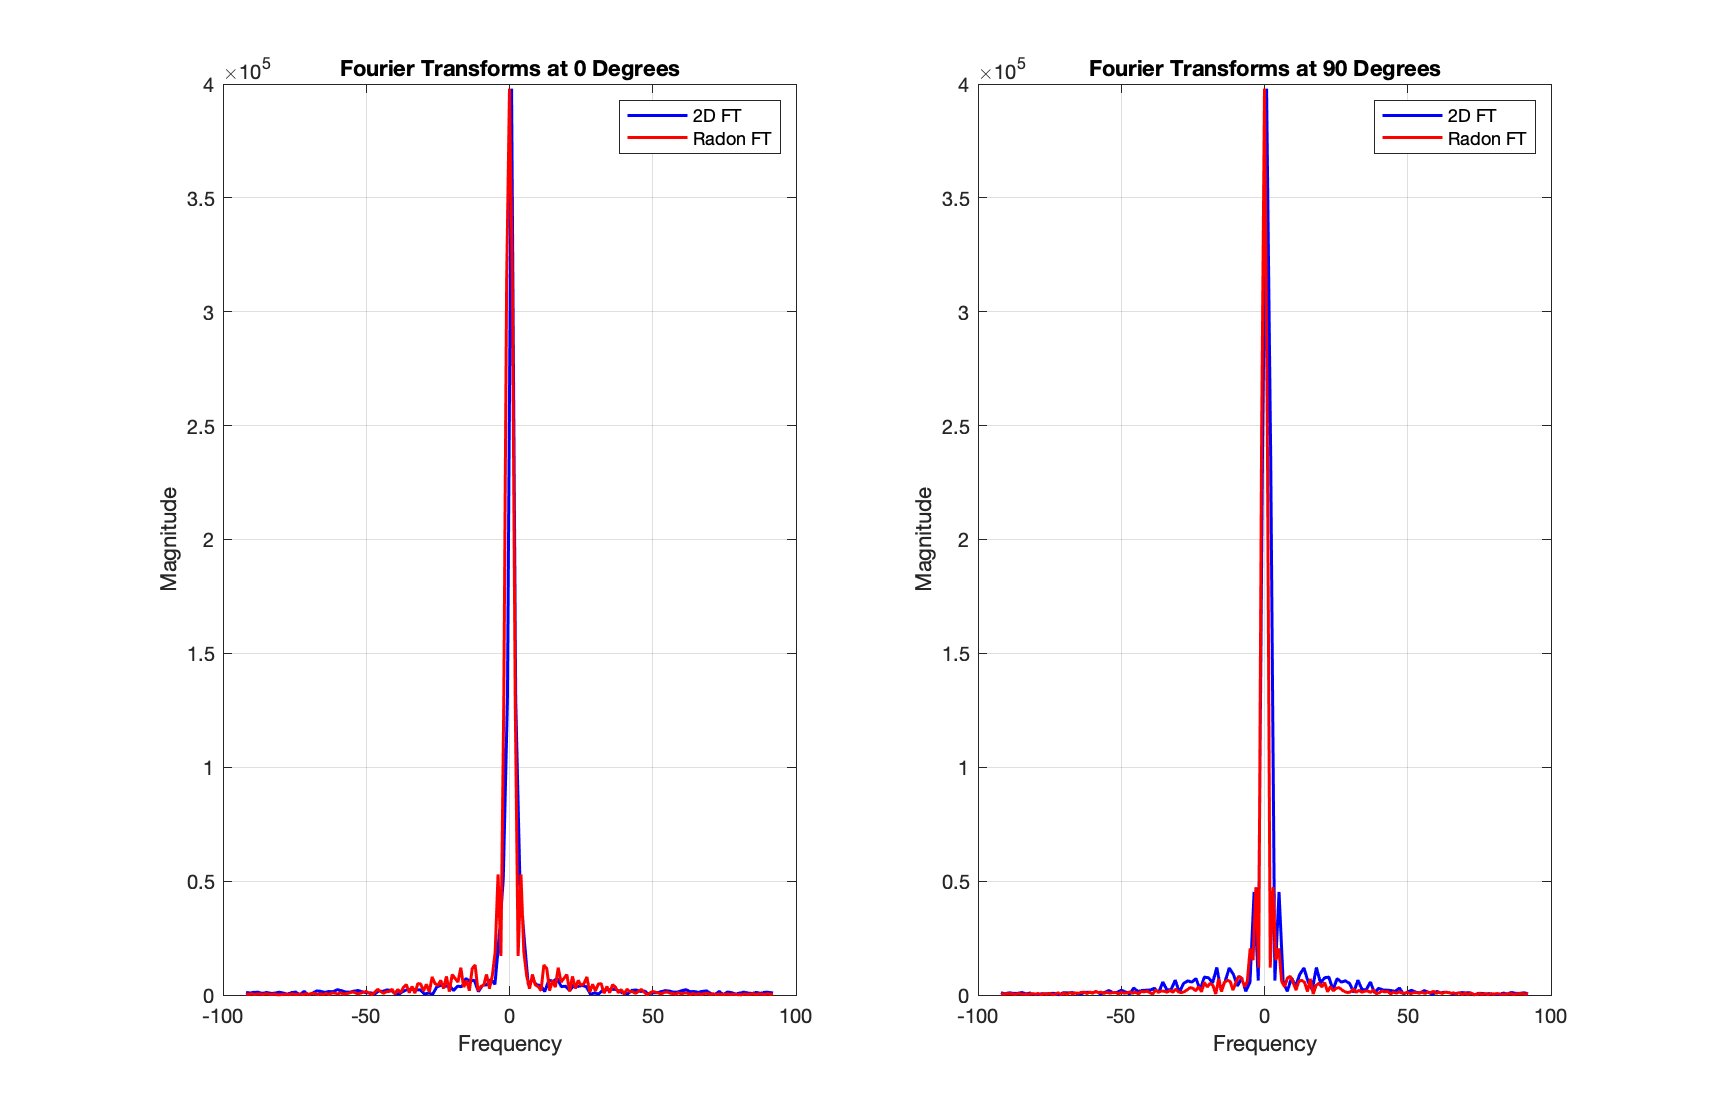
\includegraphics[width=400pt]{fig1.png}
    \caption{Direct and projection-slice Fourier transforms  at 0 and 90 degrees using slice 15}
    \label{fig1}
     \end{figure}
    	
    \item Use the 1D Fourier transform on the Radon-transformed signal from slice 15 (for angles 0 and 90 degrees) and 
    compare it with the projection-slice Fourier transform of slice 20 (using the same angles and magnitude signal). 
    Plot the results and compare them with question 4.
    Make sure your code is fully documented and can be executed without error.\\
    Answer: The green and red lines do not quite overlap  compared to the previous question.
    They are the amplitude plots of  projection-slice Fourier transforms of different slices and we can expect differences in the amplitude of the signals.
    \begin{figure}[H]
    \centering
    \captionsetup{justification=raggedright,singlelinecheck=false}
    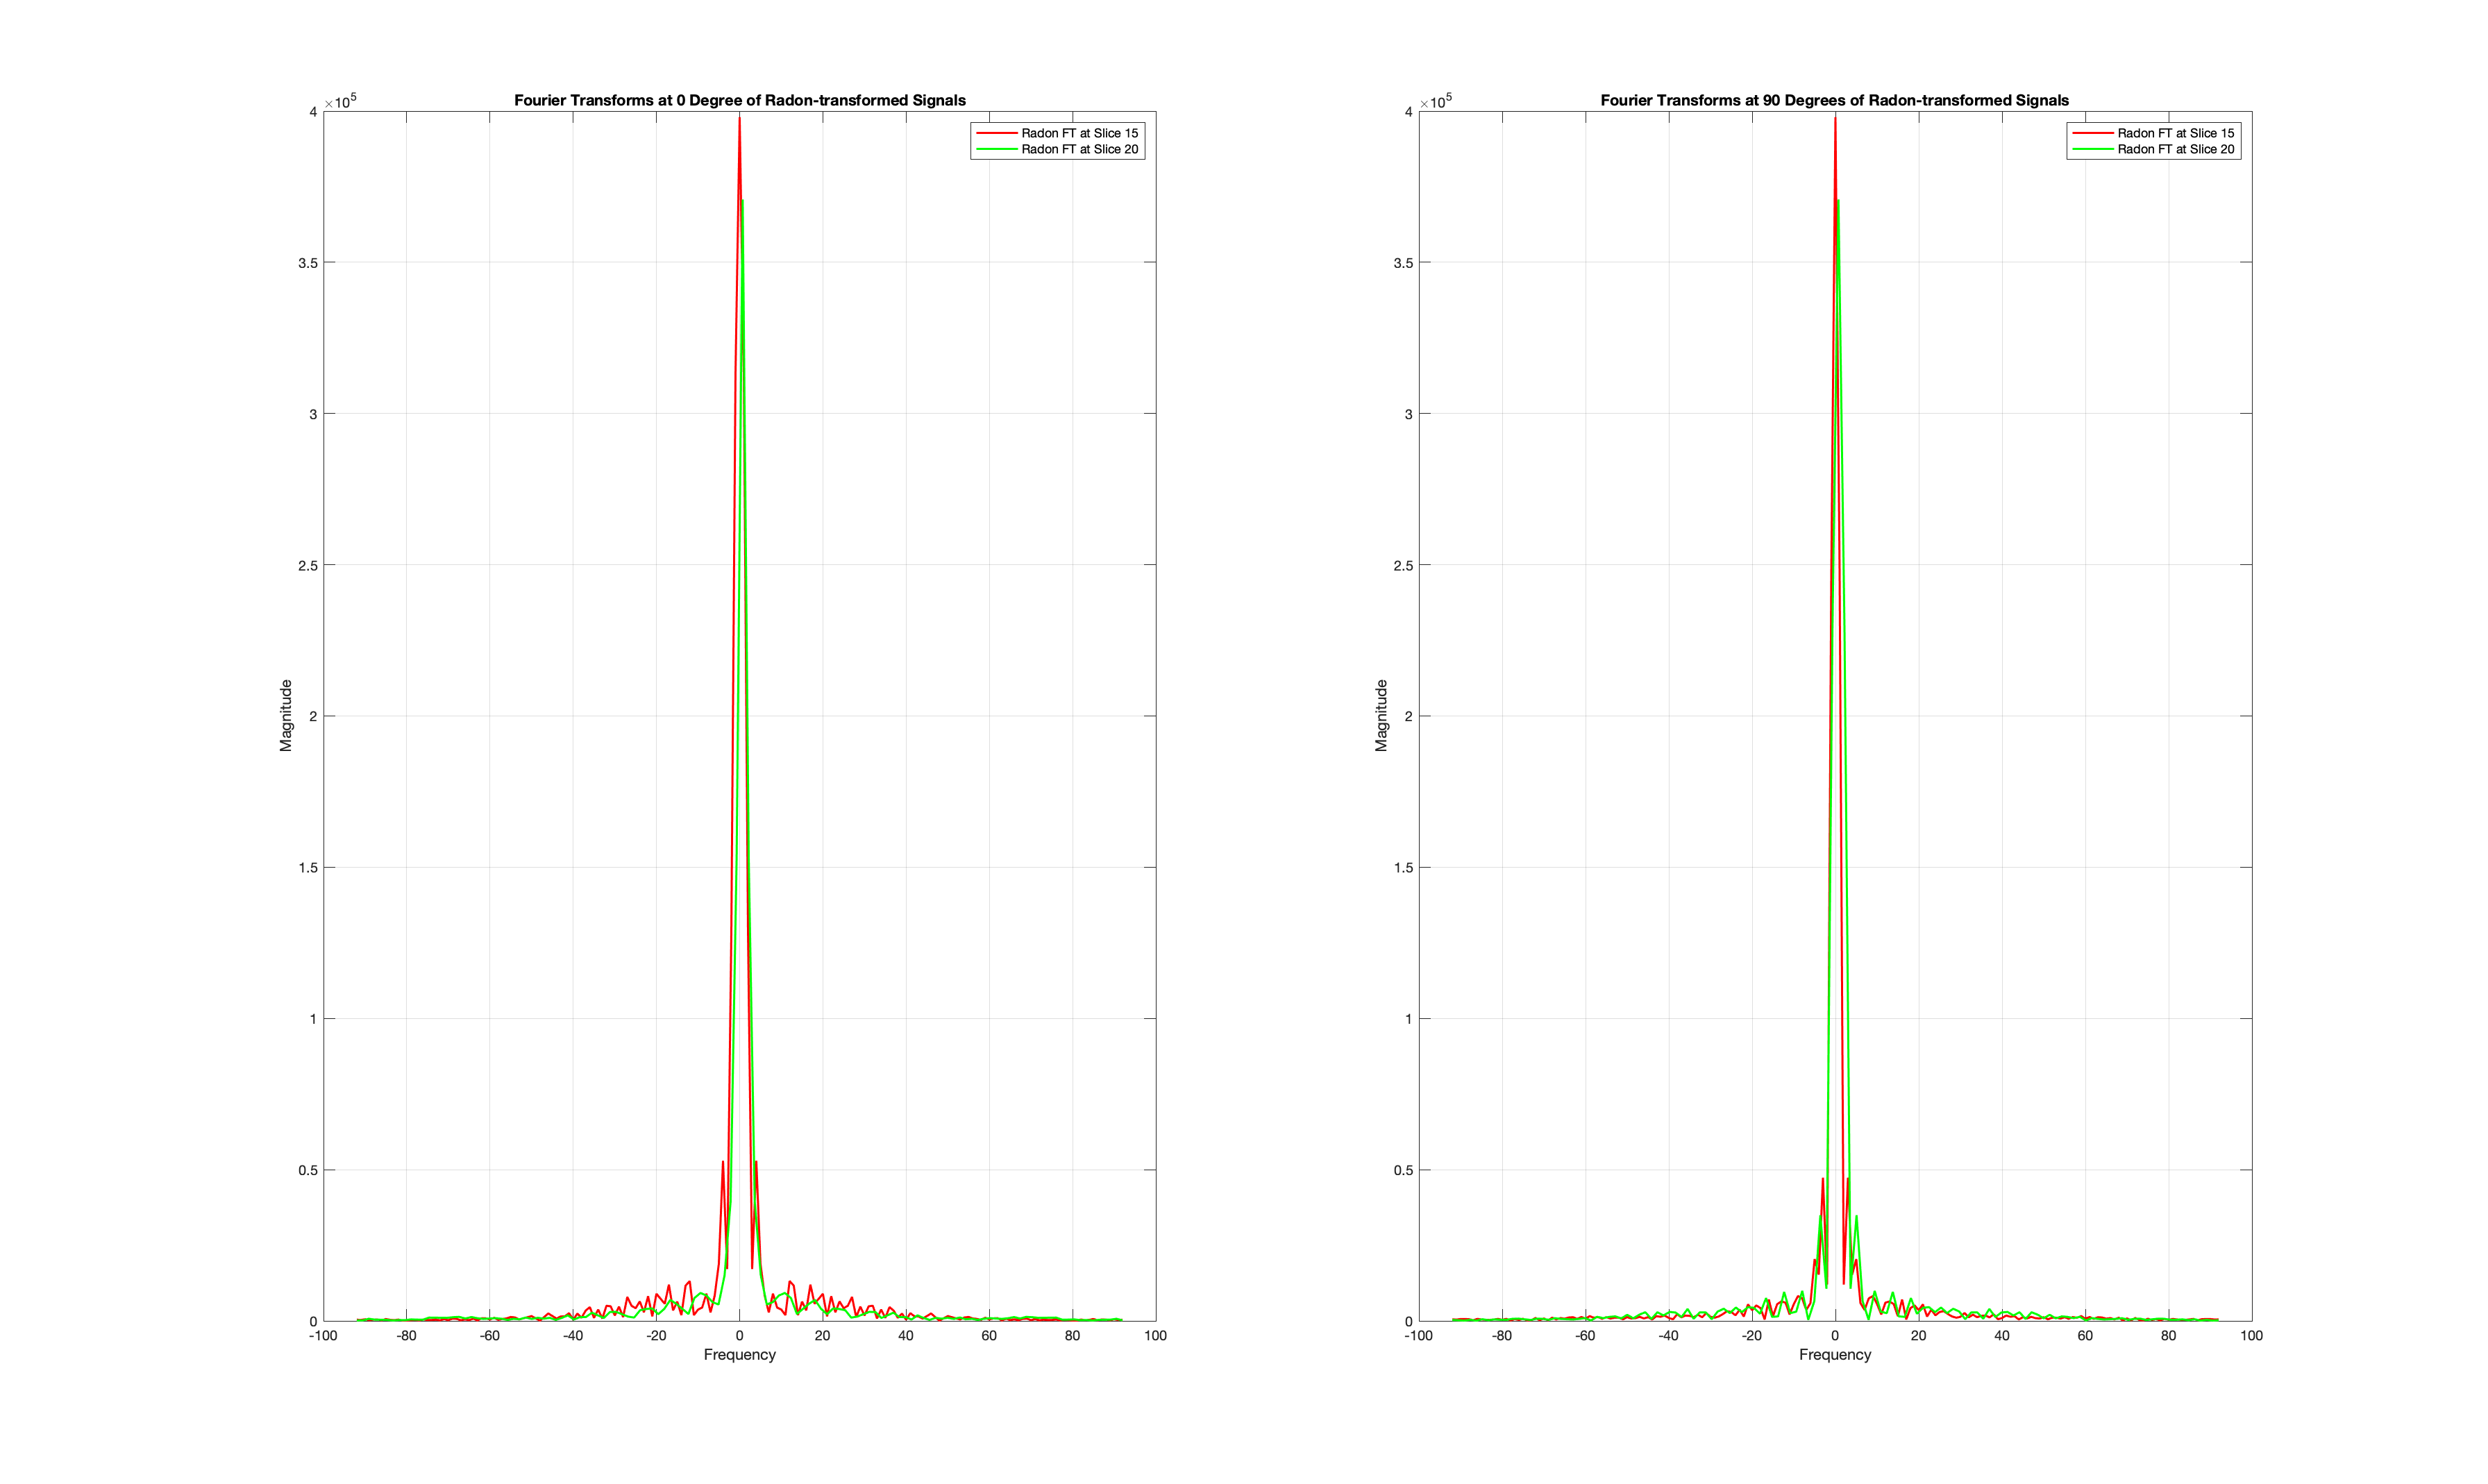
\includegraphics[width=400pt]{fig2.png}
    \caption{Projection-slice Fourier transforms at 0 and 90 degrees using slice 15 and 20}
    \label{fig2}
     \end{figure}
    \end{enumerate}

\end{document}
